% % -*- coding:utf-8 -*-
\documentclass[aspectratio=169,10pt]{beamer}
\nonstopmode

\usepackage{pifont}
\usepackage{subcaption}
\usepackage{fontawesome}
\usepackage{graphicx}
\usepackage{url}
\usepackage{enumitem}
\usepackage{caption}
\usepackage[style=authoryear,backend=biber]{biblatex}
\addbibresource{bibliography.bib}

\captionsetup{skip=4pt}
% color palette
\definecolor{tu01}{HTML}{84B818}
\definecolor{tu02}{HTML}{D18B12}
\definecolor{tu03}{HTML}{1BB5B5}
\definecolor{tu04}{HTML}{F85A3E}
\definecolor{tu05}{HTML}{4B6CFC}
\definecolor{tu06}{HTML}{E3B505}
\definecolor{tu07}{HTML}{AF331D}
\definecolor{tu08}{HTML}{000000}
\definecolor{tu09}{HTML}{AAAAAA}
\definecolor{tu10}{HTML}{444444}
\definecolor{tu11}{HTML}{84B818}

% mixed and light colors
\colorlet{tu01light}{tu01!33}
\colorlet{tu02light}{tu02!33}
\colorlet{tu03light}{tu03!33}
\colorlet{tu04light}{tu04!33}
\colorlet{tu05light}{tu05!33}
\colorlet{tu06light}{tu06!33}
\colorlet{tu07light}{tu07!33}
\colorlet{tu08light}{tu08!33}
\colorlet{tu09light}{tu09!33}
\colorlet{tu10light}{tu10!33}
\colorlet{tu11light}{tu11!33}

\colorlet{tu01midlight}{tu01!50}
\colorlet{tu02midlight}{tu02!50}
\colorlet{tu03midlight}{tu03!50}
\colorlet{tu04midlight}{tu04!50}
\colorlet{tu05midlight}{tu05!50}
\colorlet{tu06midlight}{tu06!50}
\colorlet{tu07midlight}{tu07!50}
\colorlet{tu08midlight}{tu08!50}
\colorlet{tu09midlight}{tu09!50}
\colorlet{tu10midlight}{tu10!50}
\colorlet{tu11midlight}{tu11!50}

\colorlet{tu01dark}{tu01!80!black}
\colorlet{tu02dark}{tu02!80!black}
\colorlet{tu03dark}{tu03!80!black}
\colorlet{tu04dark}{tu04!80!black}
\colorlet{tu05dark}{tu05!80!black}
\colorlet{tu06dark}{tu06!80!black}
\colorlet{tu07dark}{tu07!80!black}
\colorlet{tu08dark}{tu08!80!black}
\colorlet{tu09dark}{tu09!80!black}
\colorlet{tu10dark}{tu10!80!black}
\colorlet{tu11dark}{tu11!80!black}

\colorlet{lightgray}{gray!25}
\colorlet{midlightgray}{gray!50}
\colorlet{anthracite}{black!85}

% aliases
\colorlet{tudo}{tu01}
\colorlet{tuorange}{tu02}
\colorlet{tudolight}{tu01light}

% \usepackage{beamerthememetropolis}
\usetheme[progressbar=frametitle]{metropolis}
\metroset{progressbar=none}
\newcommand{\themename}{\textbf{\textsc{metropolis}}\xspace}


\usepackage{xcolor}
% Remove default navigation symbols
\setbeamertemplate{navigation symbols}{}
\setbeamercolor{background canvas}{bg=white}

% Custom footline with frame numbers on the left and navigation symbols on the right
\setbeamertemplate{footline}{
  \leavevmode%
  \hbox{%
    \begin{beamercolorbox}[wd=.1\paperwidth,ht=2.5ex,dp=1.125ex,leftskip=1em,rightskip=1em]{author in head/foot}%
      \usebeamerfont{footline} \insertframenumber{} / \inserttotalframenumber
    \end{beamercolorbox}%
    \hfill
    \begin{beamercolorbox}[wd=.9\paperwidth,ht=2.5ex,dp=1.125ex,leftskip=1em,rightskip=1em]{author in head/foot}%
      \usebeamerfont{footline} %\insertnavigation{2cm}
    \end{beamercolorbox}%
  }%
  \vskip0pt%
}


\title{Development of an open-source calibration framework\\ for superconducting qubits}
\subtitle{Master degree in Physics}
\author{Elisa Stabilini}
\institute{Università degli Studi di Milano - Department of Physics}
\titlegraphic{\hfill}
\date{July 4th 2025}

\begin{document}

\maketitle

\begin{frame}{Table of contents}
    \setbeamertemplate{section in toc}[sections numbered]
    \setbeamertemplate{subsection in toc}[subsections numbered]  
    \tableofcontents[hideallsubsections]
\end{frame}

\begin{frame}[t,fragile]{Qibo framework}
  \begin{center}
      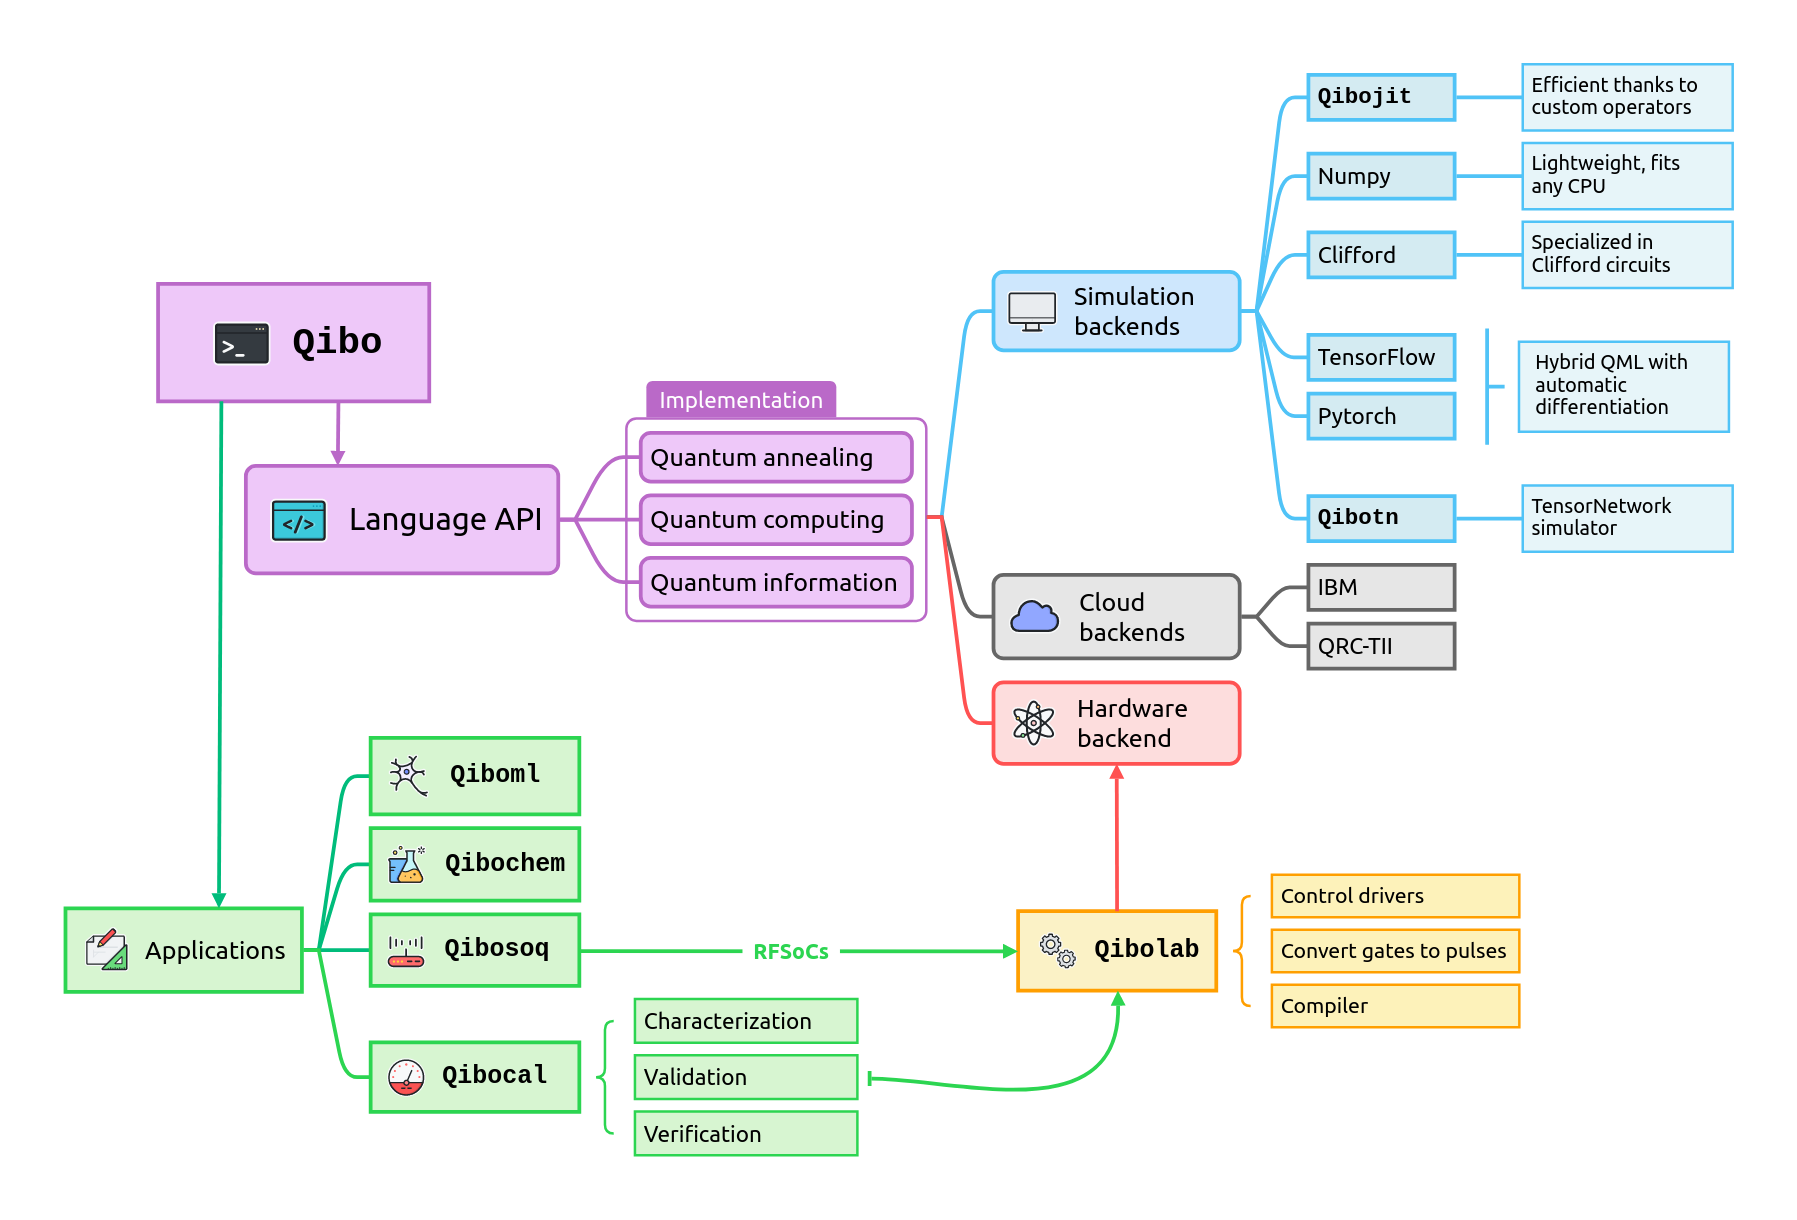
\includegraphics[height=0.80\paperheight]{figures/qibo_ecosystem.png}
  \end{center}
\end{frame}

\section{Superconducting qubits}

\begin{frame}{Artificial atoms}
  \begin{columns}
    \begin{column}{0.6\textwidth}
      \centering
      \begin{itemize}
        \item Qubit: two level system
        \hspace{10 mm}
        \item Superconducting qubits: use Josephson Junctions\\ to build anharmonic oscillators
      \end{itemize}
      \begin{figure}
        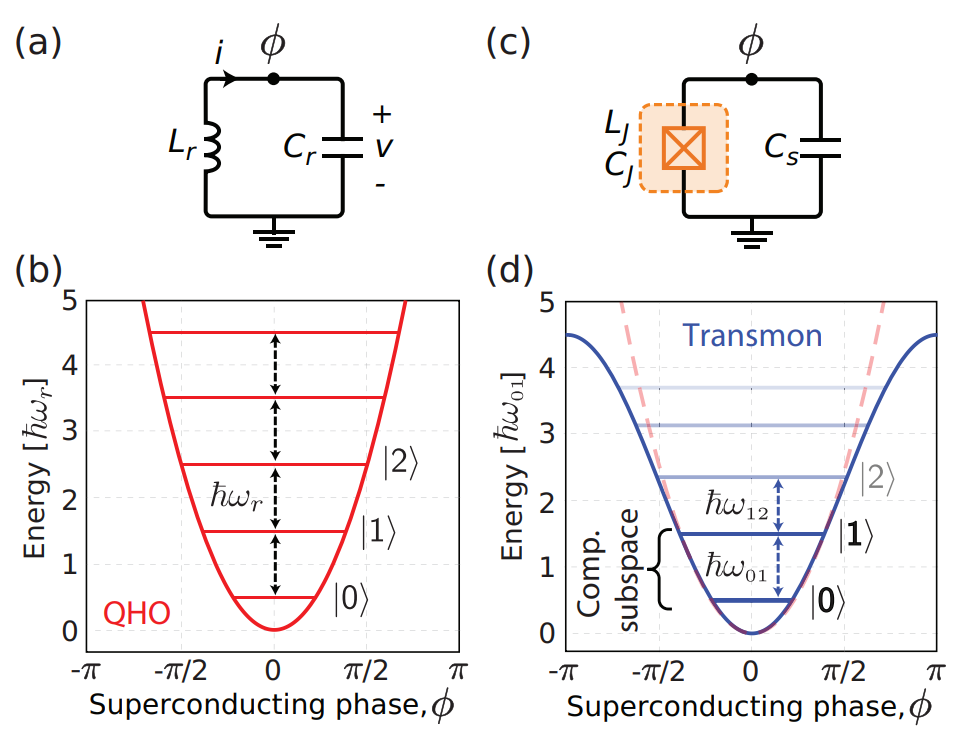
\includegraphics[height=0.5\textheight]{figures/Transmon.png}
        \caption{DOI: 10.1109/MAP.2022.3176593}
      \end{figure}
    \end{column}
    \begin{column}{0.6\textwidth}
      \centering
      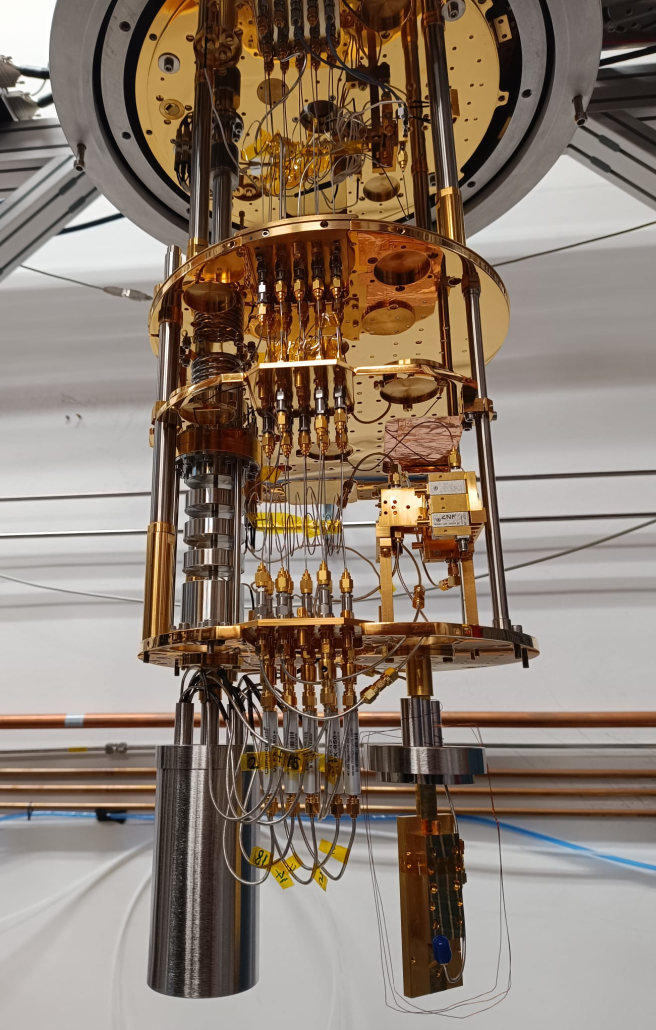
\includegraphics[width=0.5\textwidth]{figures/cryostat.png}
    \end{column}
  \end{columns}
\end{frame}

\begin{frame}{Qubit control}

  Electromagnetic pulse applied to the qubit
  \begin{equation*}
    V_d(t) = A\varepsilon(t)\sin{(\omega_d t + \alpha)},
  \end{equation*}

  Qubit - electric field Hamiltonian (RWA)
  \begin{equation*}
    \hat{H} = -\frac{\hbar (\omega_q - \omega_d)}{2} \hat{\sigma}_z + \frac{\hbar \Omega}{2} \varepsilon(t) \left( \hat{\sigma}_x \cos \alpha + \hat{\sigma}_y \sin \alpha \right),
  \end{equation*}

  General qubit evolution under electromagnetic pulse:
  \begin{equation*}
    R_{\hat{n}(\alpha)}(\theta) = e^{-\frac{i}{2} \hat{n}(\alpha) \cdot \vec{\sigma} \theta} = e^{-\frac{i}{2} (\hat{\sigma}_x \cos \alpha + \hat{\sigma}_y \sin \alpha) \theta},
  \end{equation*}

  where $\theta = \Omega\int_{0}^{+\infty}\varepsilon(t')dt'$

\end{frame}

\begin{frame}{State readout}
  \begin{columns}
    \begin{column}{0.35\textwidth}
    Qubit - resonator Hamiltonian:
    \begin{equation*}
      \hat{H} = \hbar\omega_r\hat{a}\hat{a}^\dagger - \frac{\hbar\omega_{01}}{2}\hat{\sigma}_z + \hbar g(\hat{\sigma}^+\hat{a}+\hat{\sigma}^-\hat{a}^\dagger)
    \end{equation*}\\
    \vspace{1.5em}
    Dispersive regime ($g \ll \omega_q - \omega_r$):
    \begin{equation*}
      \hat{H}_{disp} = \hbar(\omega_r - \chi\hat{\sigma}_z)\hat{a}^\dagger\hat{a} - \frac{\hbar}{2}(\omega_{01}+\chi)\hat{\sigma}_z
    \end{equation*}
    dispersive shift: $\chi = \frac{g^2}{\Delta},$ \hfill $\Delta = \omega_q - \omega_r$
  \end{column}
    \begin{column}{0.65\textwidth}
      \begin{center}
        \begin{figure}
          \vspace{2mm}
          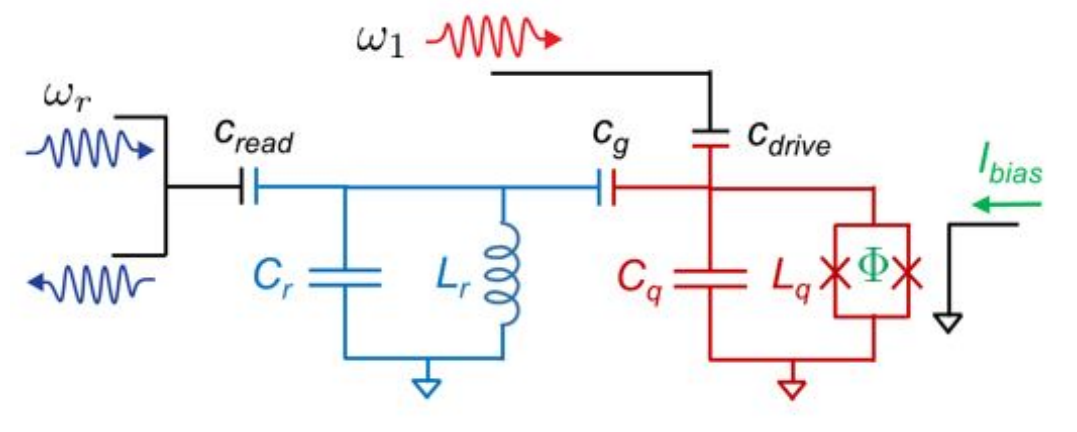
\includegraphics[width=0.85\textwidth]{figures/TransmonCircuit.png}
          \vfill
          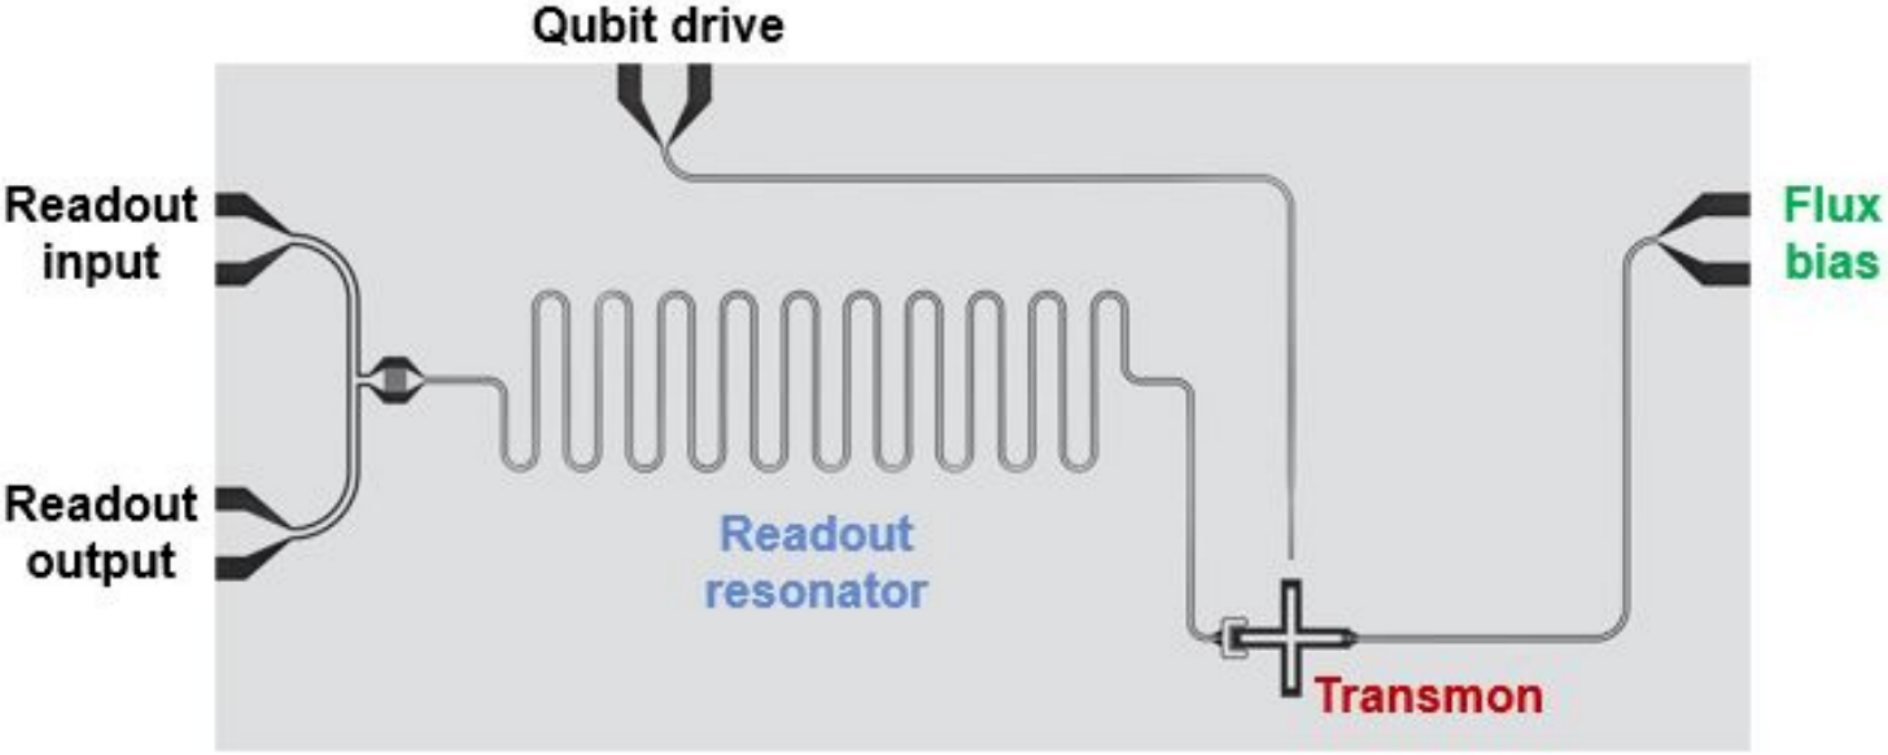
\includegraphics[width=0.85\textwidth]{figures/TransmonBoard.png}
          \caption{DOI: 10.1109/MAP.2022.3176593}
        \end{figure}
      \end{center}
    \end{column}
  \end{columns}
\end{frame}

\begin{frame}{Superconducting qubit calibration}
  \vbox to \textheight{ 
    \vspace{1em}
    \begin{minipage}[t]{\textwidth}
      \centering
      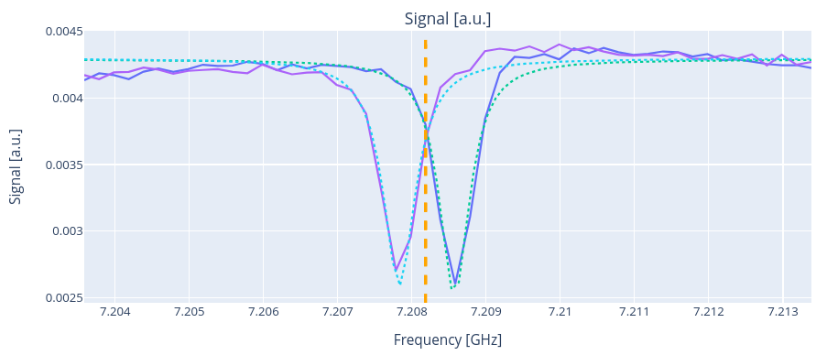
\includegraphics[height=0.4\textheight]{figures/disp_sihft.png}
      \hspace{10mm}
      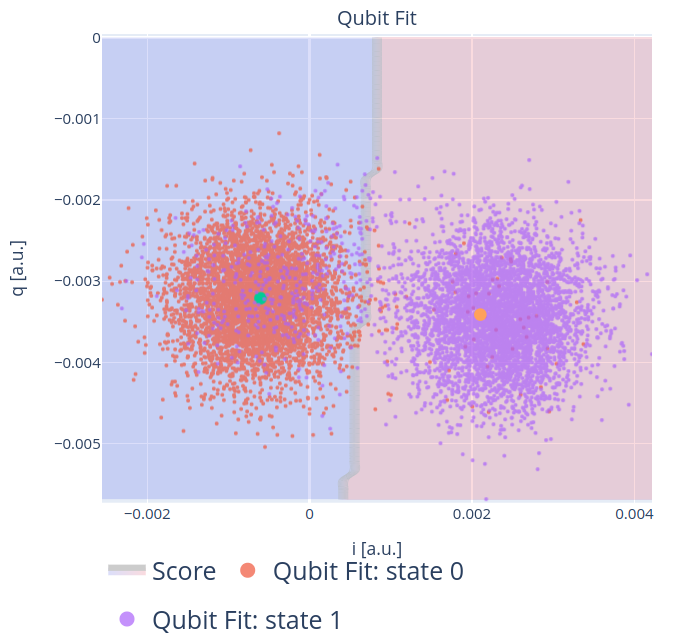
\includegraphics[height=0.4\textheight]{figures/classification.png}
    \end{minipage}
    \vspace{0.015mm}

    \begin{minipage}[b]{\textwidth}
      \centering
      \begin{columns}
        \begin{column}{0.4\textwidth}
          Procedure:
          \setbeamertemplate{enumerate items}[default]
          \begin{enumerate}[leftmargin=*, label=\arabic*.]
            \item Resonator characterization
            \item Qubit characterization
            \item Gate calibration
            \item Gate set characterization
          \end{enumerate}
        \end{column}
        \begin{column}{0.4\textwidth}
          Metrics example:
          \begin{itemize}[label={\raisebox{0.2ex}{\tiny$\bullet$}}]
            \item readout \& assignment fidelity
            \item relaxation time $T_1$
            \item decoherence time $T_22$
            \item gate fidelity
          \end{itemize}   
        \end{column}
      \end{columns}
    \end{minipage}
    \vspace{1em}
  }
\end{frame}

\begin{frame}{Superconducting qubit calibration}
  \vbox to \textheight{ 
    \vspace{1em}
    \begin{minipage}[t]{\textwidth}
      \centering
      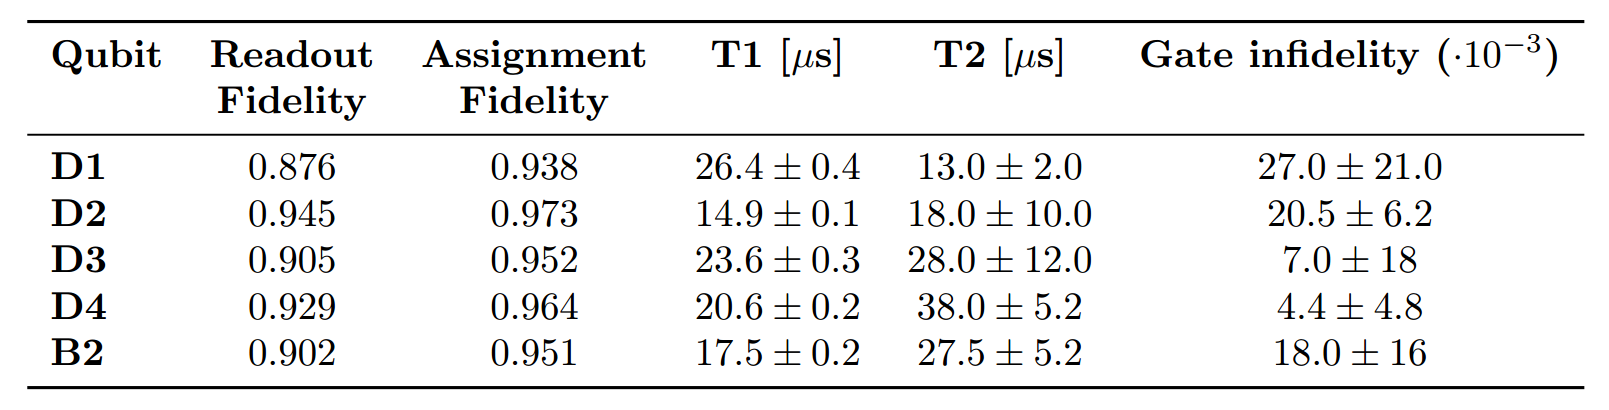
\includegraphics[height=0.4\textheight]{figures/cal_results.png}
    \end{minipage}
    \vspace{0.015mm}

    \begin{minipage}[b]{\textwidth}
      \centering
      \begin{columns}
        \begin{column}{0.4\textwidth}
          Procedure:
          \setbeamertemplate{enumerate items}[default]
          \begin{enumerate}[leftmargin=*, label=\arabic*.]
            \item Resonator characterization
            \item Qubit characterization
            \item Gate calibration
            \item Gate set characterization
          \end{enumerate}
        \end{column}
        \begin{column}{0.4\textwidth}
          Metrics example:
          \begin{itemize}[label={\raisebox{0.2ex}{\tiny$\bullet$}}]
            \item readout \& assignment fidelity
            \item relaxation time $T_1$
            \item decoherence time $T_22$
            \item gate fidelity
          \end{itemize}   
        \end{column}
      \end{columns}
    \end{minipage}
    \vspace{1em}
  }
\end{frame}

\section{Average Clifford gate fidelity optimization}

\begin{frame}[t,fragile]{Randomized Benchmarking}
\begin{center}
  Randomized benchmarking estimates average gate fidelity by applying random sequences of Clifford gates followed by an inverting gate.
  \vspace{3mm}
  \begin{figure}
      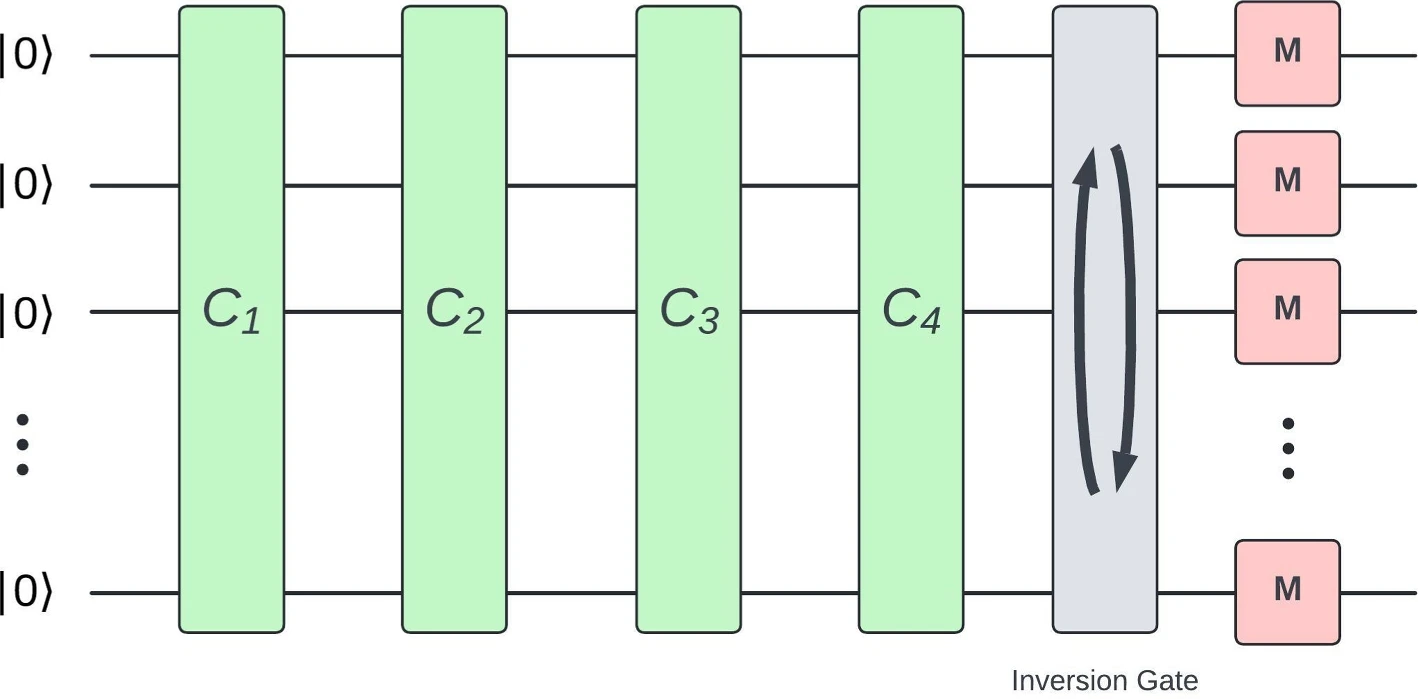
\includegraphics[height=0.52\textheight]{figures/RBcircuit.png}
      \caption{DOI: 10.1007/s10773-024-05811-8}
  \end{figure}
\end{center}
\end{frame}

\begin{frame}[t,fragile]{Randomized Benchmarking}
\begin{center}
  Randomized benchmarking estimates average gate fidelity by applying random sequences of Clifford gates followed by an inverting gate.
  \vfill
  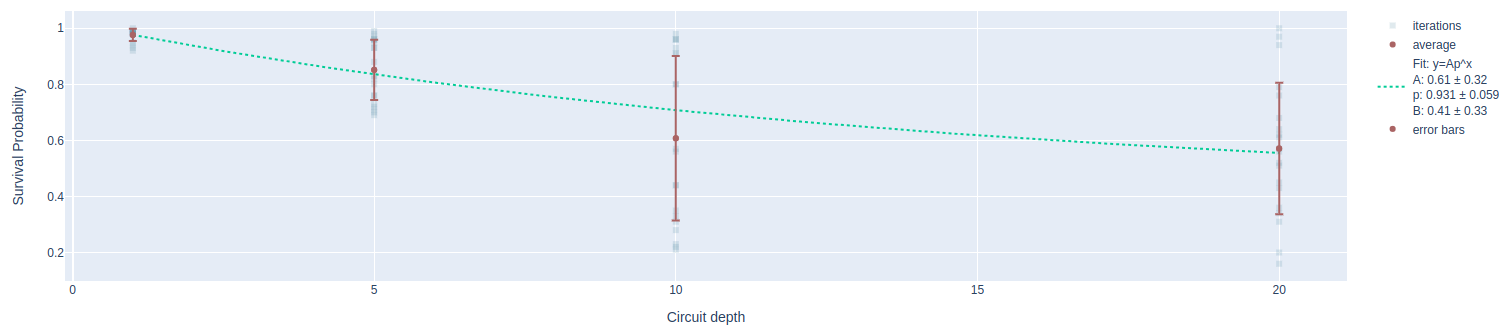
\includegraphics[width=\textwidth]{figures/rb.png}
\end{center}
\end{frame}

\begin{frame}[t,fragile]{Randomized Benchmarking}
\begin{center}
  Randomized benchmarking estimates average gate fidelity by applying random sequences of Clifford gates followed by an inverting gate.
  \vspace{1.25em}

  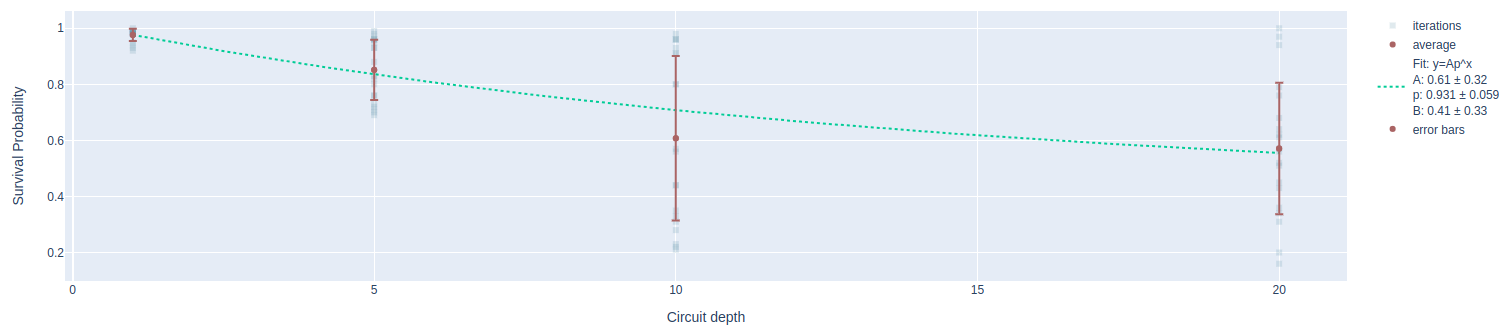
\includegraphics[width=\textwidth]{figures/rb.png}
  \vspace{1.25em}
  Can we optimize the average gate fidelity to automate $RX$ gate reacalibration? 
\end{center}
\end{frame}

\begin{frame}[t,fragile]{RB optimization [\cite{kelly_optimal_2014}]}
  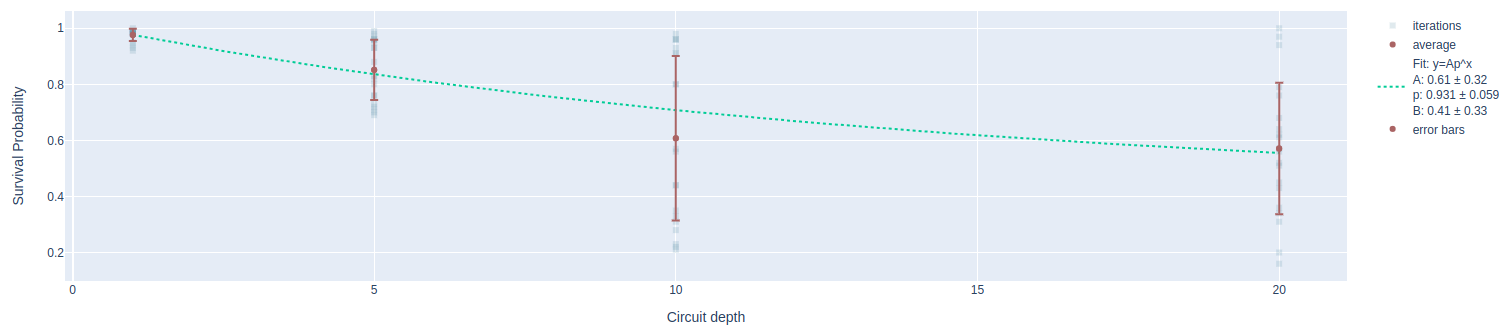
\includegraphics[width=\textwidth]{figures/rb.png}\\
  \vspace{1em}
  Can we optimize the average gate fidelity to automate $RX$ gate reacalibration?\\
  \vspace{1em}
  Test closed-loop optimization with modern optimization libraries\\

  \vspace{1em}
  Optimization parameters: \; \textbf{amplitude}, \; \textbf{frequency} \; \textbf{$\beta$ DRAG parameter}
\end{frame}


\begin{frame}[t,fragile]{Average Clifford gate Fidelity}
    \vbox to \textheight{ 
    \vspace{1em}
    \begin{minipage}[t]{\textwidth}
      \centering
      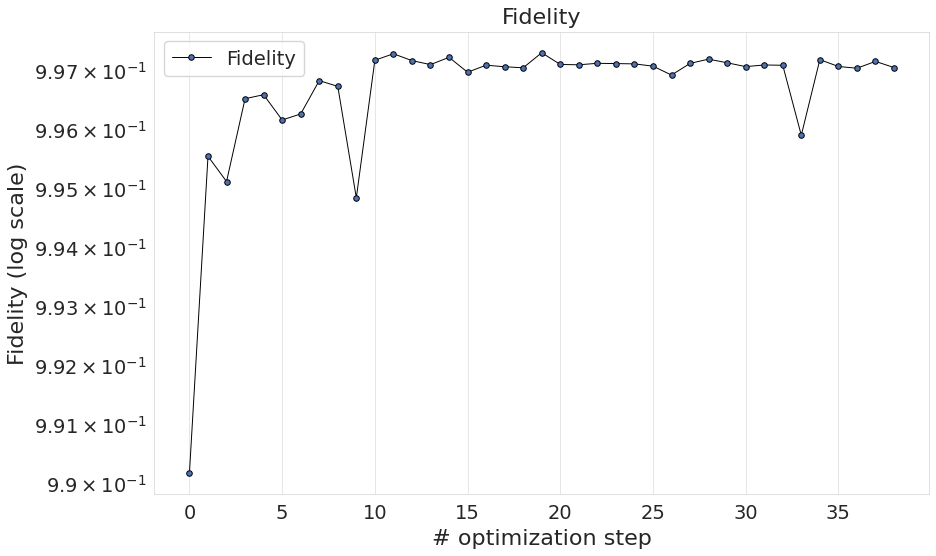
\includegraphics[height=0.35\textheight]{figures/NM_fid.png}
      \hspace{10mm}
      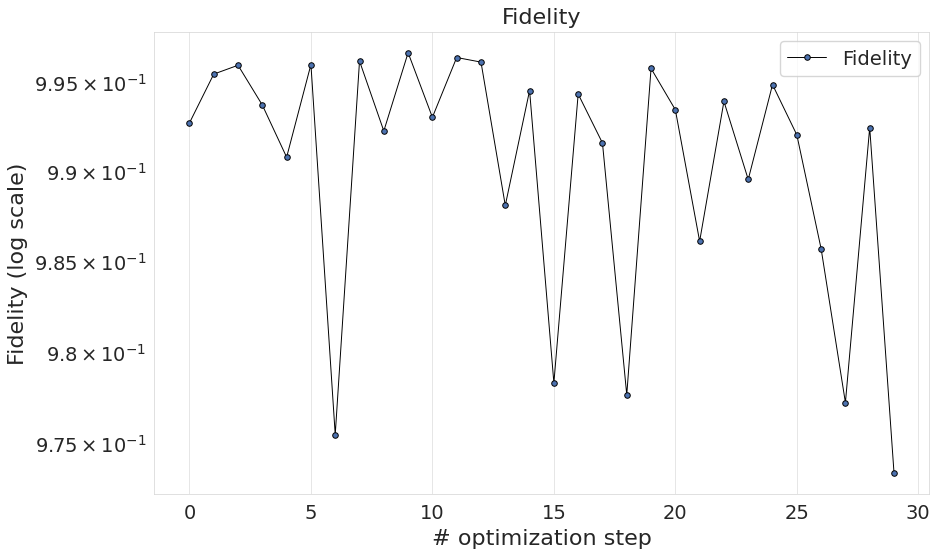
\includegraphics[height=0.35\textheight]{figures/fidelity_CMA.png}
    \end{minipage}
    \vspace{0.5em}
    \begin{minipage}[b]{\textwidth}
      \centering
      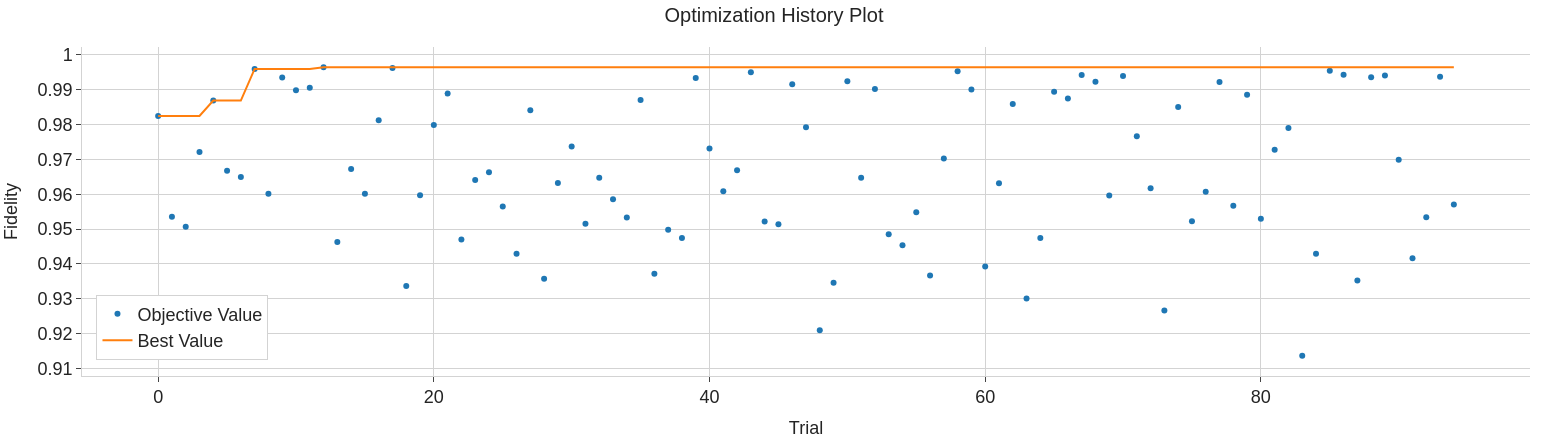
\includegraphics[width=0.85\textwidth]{figures/optuna.png}
    \end{minipage}
    \vspace{1em}
  }
\end{frame}

\begin{frame}[t,fragile]{Parameters evolution}
  \begin{figure}
    \begin{subfigure}[t]{0.315\textwidth}
      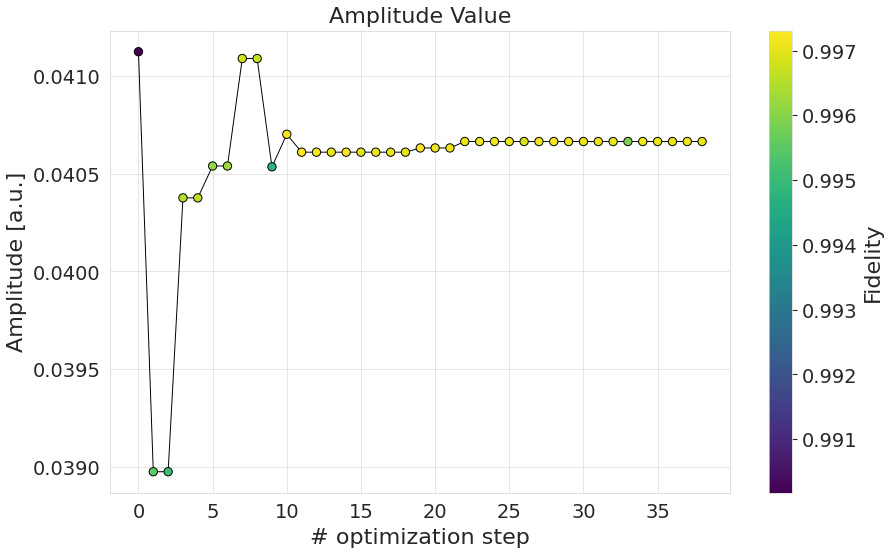
\includegraphics[width=\textwidth]{figures/amplitude.png}
    \end{subfigure}
        \begin{subfigure}[t]{0.315\textwidth}
      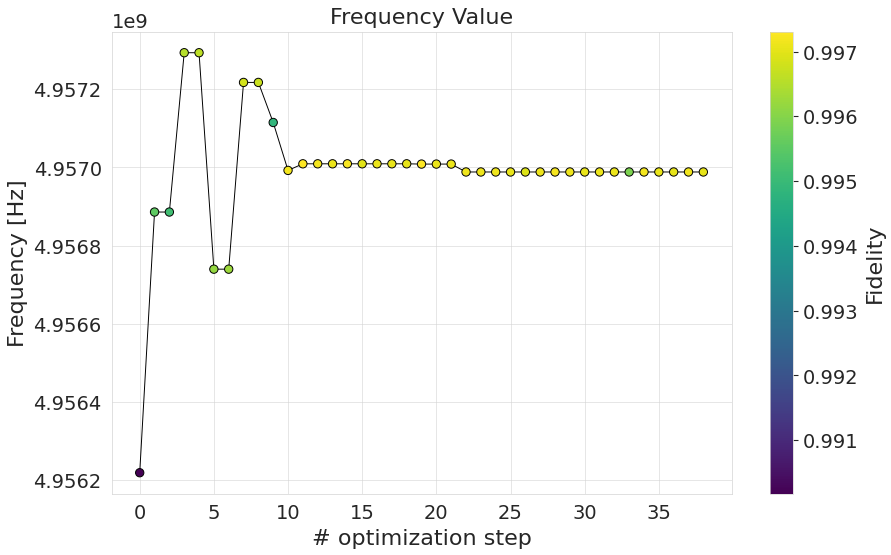
\includegraphics[width=\textwidth]{figures/frequency.png}
    \end{subfigure}
        \begin{subfigure}[t]{0.315\textwidth}
      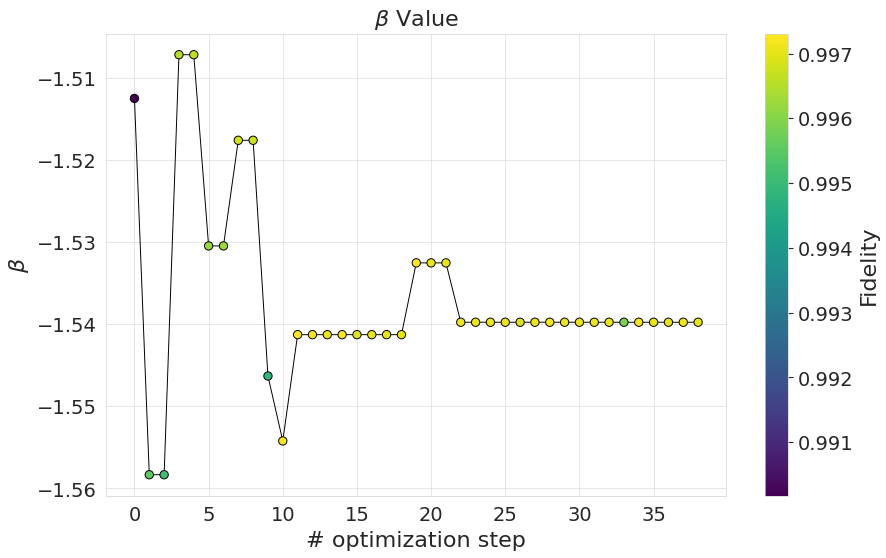
\includegraphics[width=\textwidth]{figures/beta.png}
    \end{subfigure}

  \end{figure}
    \begin{figure}
    \begin{subfigure}[t]{0.315\textwidth}
      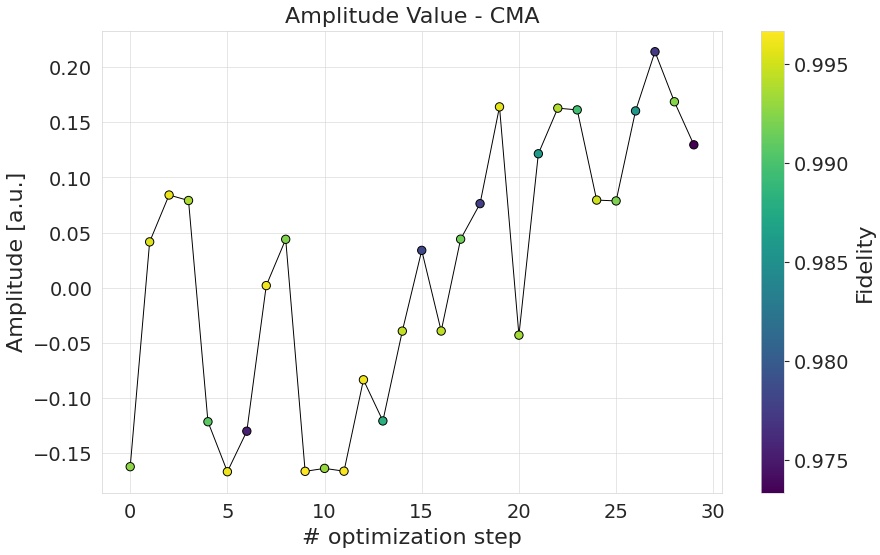
\includegraphics[width=\textwidth]{figures/CMA_amplitude.png}
    \end{subfigure}
        \begin{subfigure}[t]{0.315\textwidth}
      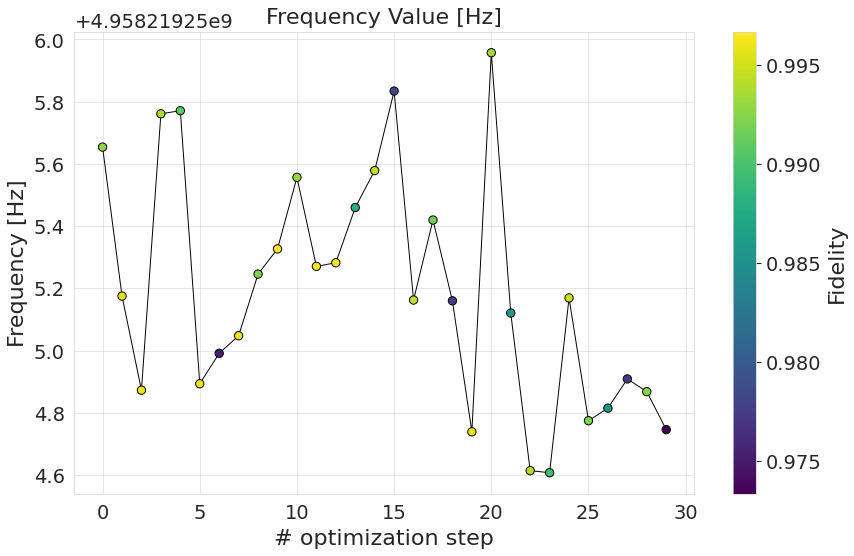
\includegraphics[width=\textwidth]{figures/CMA_frequency.png}
    \end{subfigure}
        \begin{subfigure}[t]{0.315\textwidth}
      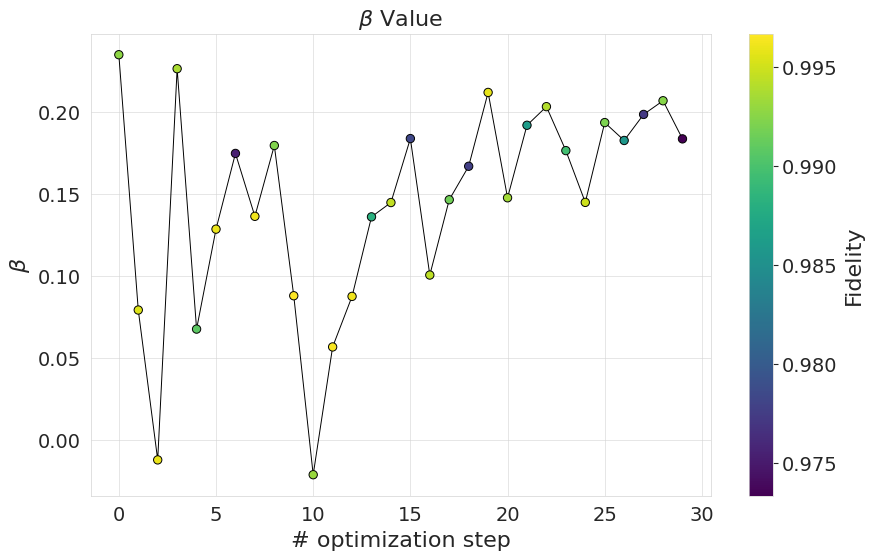
\includegraphics[width=\textwidth]{figures/beta_CMA.png}
    \end{subfigure}
  \end{figure}
\end{frame}

%\begin{frame}[t,fragile]{Results summary}
%  \begin{itemize}
%    \item[\ding{51}] Fidelity improvement
%    \item[\ding{55}]Overall time-expensive
%    \item[\ding{55}]Unstable convergence
%  \end{itemize}
%
%%  \begin{figure}
%%    \centering
%%    \includegraphics[options]{name}
%%  \end{figure}
%
%\end{frame}

\section{Library additions}
\subsection{Native RX90}

\begin{frame}{Native RX90}
  \begin{itemize}
    \item Only native gates are directly implemented on hardware, other gates are transpiled into natives
    \hspace{10 mm}
    \item Qibolab single qubit natives: $RX$, $MZ$ + $RX/2$
  \end{itemize}
\end{frame}

\begin{frame}{Native RX90}
  \begin{itemize}
    \item Only native gates are directly implemented on hardware, other gates are transpiled into natives
    \hspace{10 mm}
    \item Qibolab single qubit natives: RX, MZ
    \hspace{10 mm}
    \item Add RX90 native for more precise gates implementation
  \end{itemize}
  \begin{figure}
    \centering
    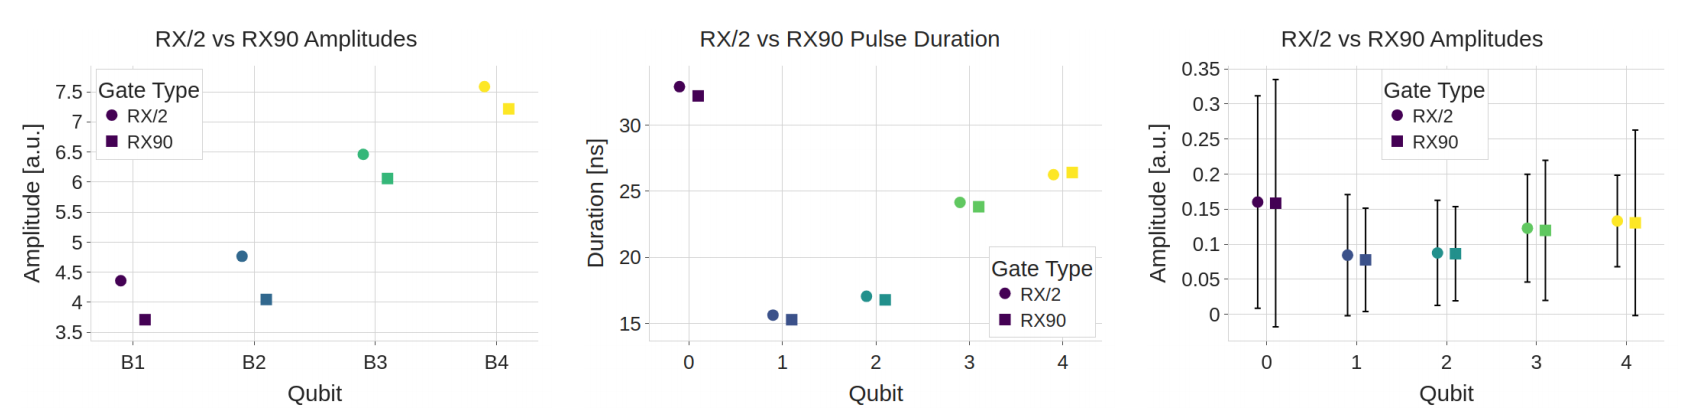
\includegraphics[width=\textwidth]{figures/RX90.png}
  \end{figure}
\end{frame}

\begin{frame}{Rabi amplitude experiment}
    \begin{figure}
    \centering
    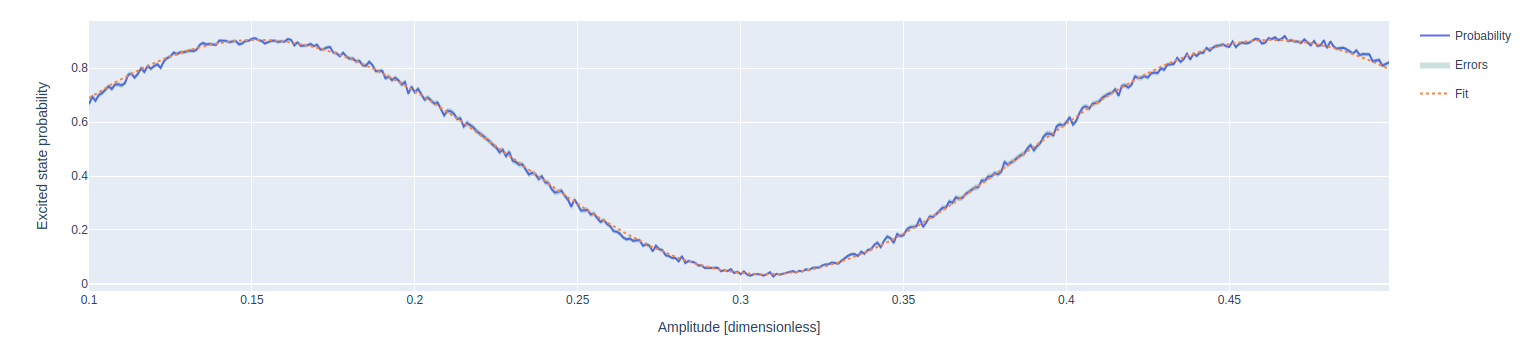
\includegraphics[width=\textwidth]{figures/B4.png}
    \vfill
    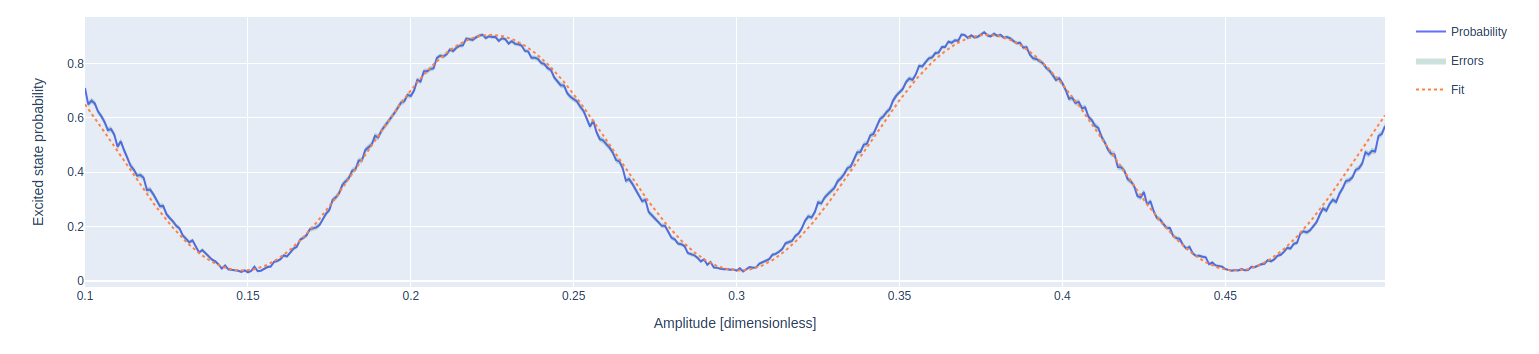
\includegraphics[width=\textwidth]{figures/B4_90.png}
  \end{figure}
\end{frame}

\subsection{Cryoscope}

\begin{frame}{Flux pulse reconstruction [\cite{rol_time-domain_2020}]}
  \begin{columns}
    \begin{column}{0.5\textwidth}
      \centering
      Transmon flux dependence:
      \begin{equation*}
        f_q(\Phi_q) \approx \left( \sqrt{8E_J E_C \left| \cos\left(\pi \frac{\Phi_q}{\Phi_0}\right) \right|} \right)
      \end{equation*}\\
      \vspace{3em}
      Detuning as function of the flux pulse:
      \begin{equation*}
        \Delta f_R = \frac{1}{\Delta \tau} \int_{\tau}^{\tau + \Delta \tau} \Delta f_q(\Phi_{q, \tau + \Delta \tau} (t))
        %TODO: riguardare notazione
      \end{equation*}
    \end{column}
    \begin{column}{0.5\textwidth}
      \begin{figure}
        \centering
        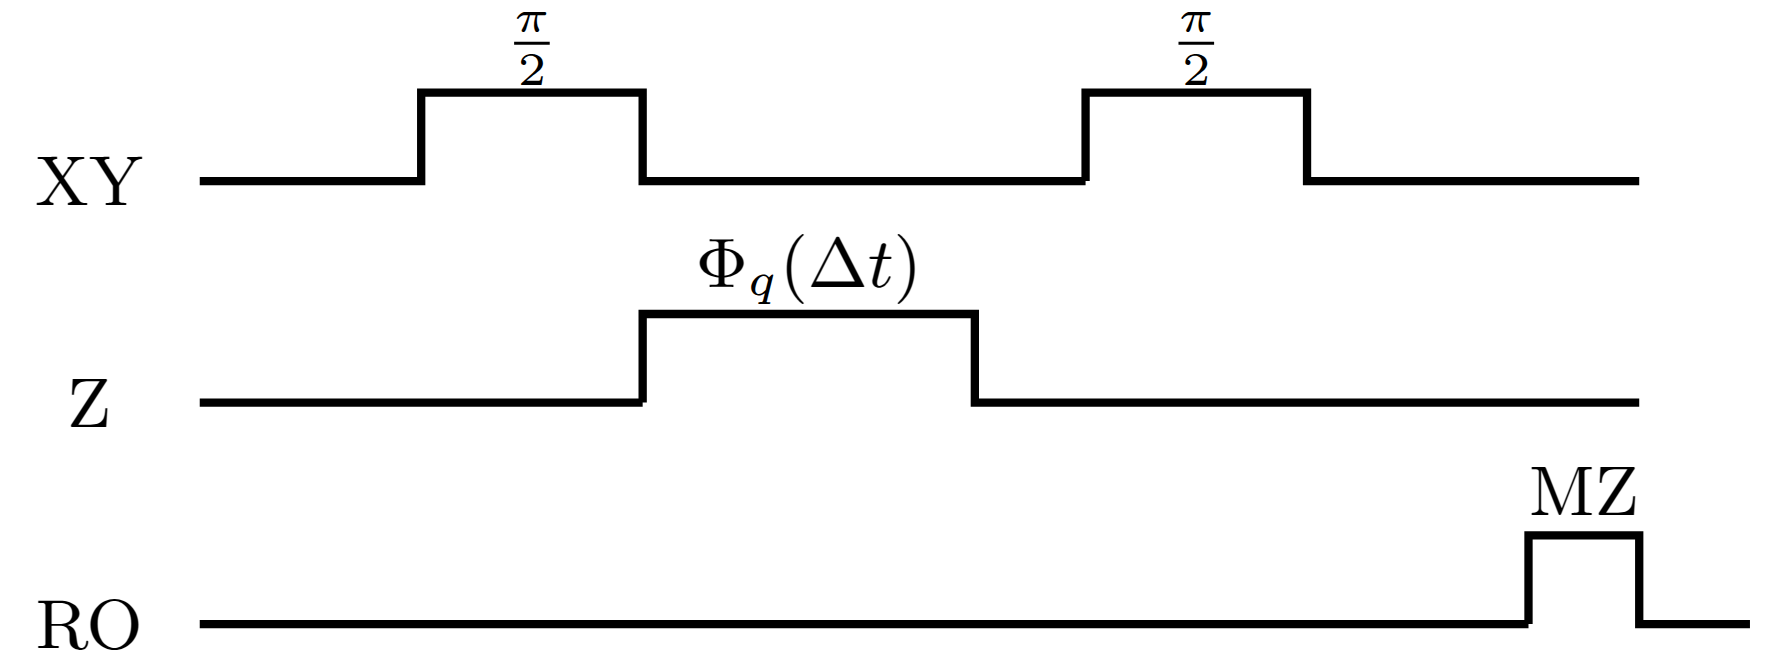
\includegraphics[width=0.85\textwidth]{figures/cryoscope_pulse.png}\\
        \vspace{3em}
        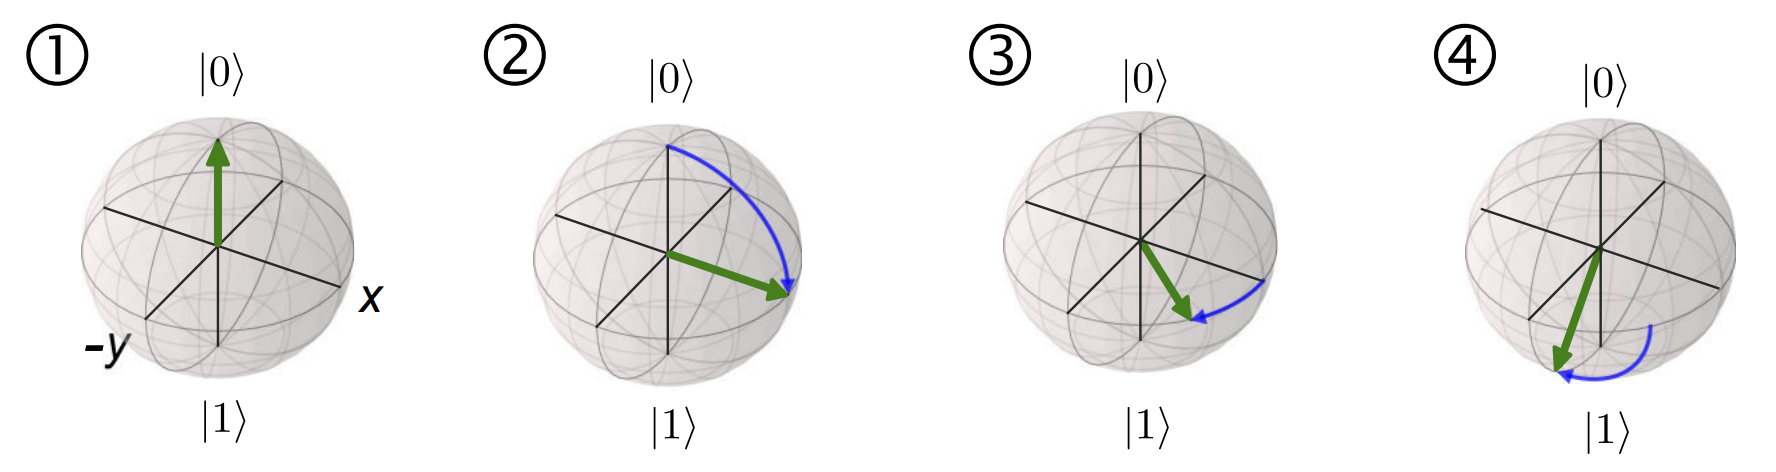
\includegraphics[width=0.85\textwidth]{figures/BlochEvolution.png}
        \caption{DOI: 10.1039/D2TC01258H}
      \end{figure}
    \end{column}
  \end{columns}
\end{frame}

\begin{frame}{Filter determination}
  \begin{figure}
    \centering
    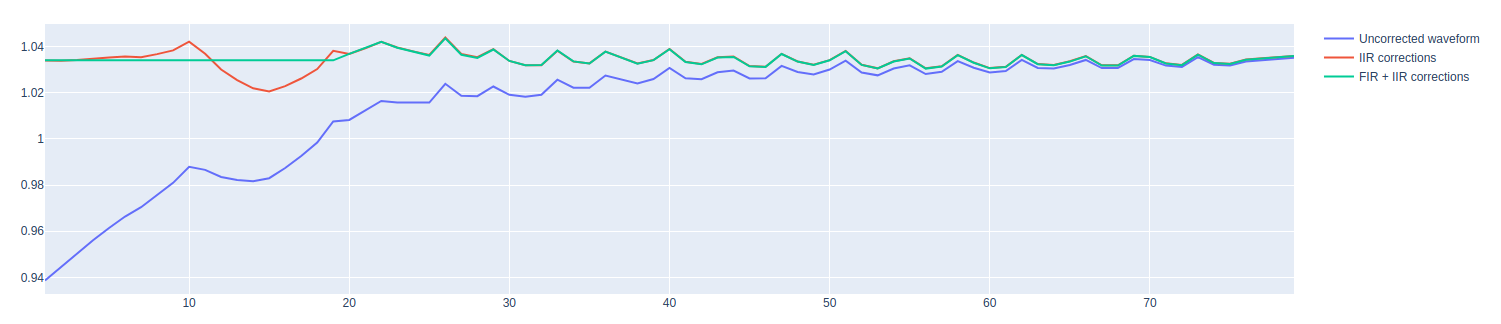
\includegraphics[width=\textwidth]{figures/B4_ringin.png}
  \end{figure}
  \vspace{0.5em}
  {\setbeamertemplate{enumerate items}[default]
    \begin{enumerate}[leftmargin=*, label=\arabic*.]    
      \item Determine exponential correction
      \item Obtain IIR filters from exponential correction
      \item Determine FIR
      \item Apply pre-distortion
    \end{enumerate}}
\end{frame}

\begin{frame}{Impact on chevron plots}
  \begin{figure}
    \centering
    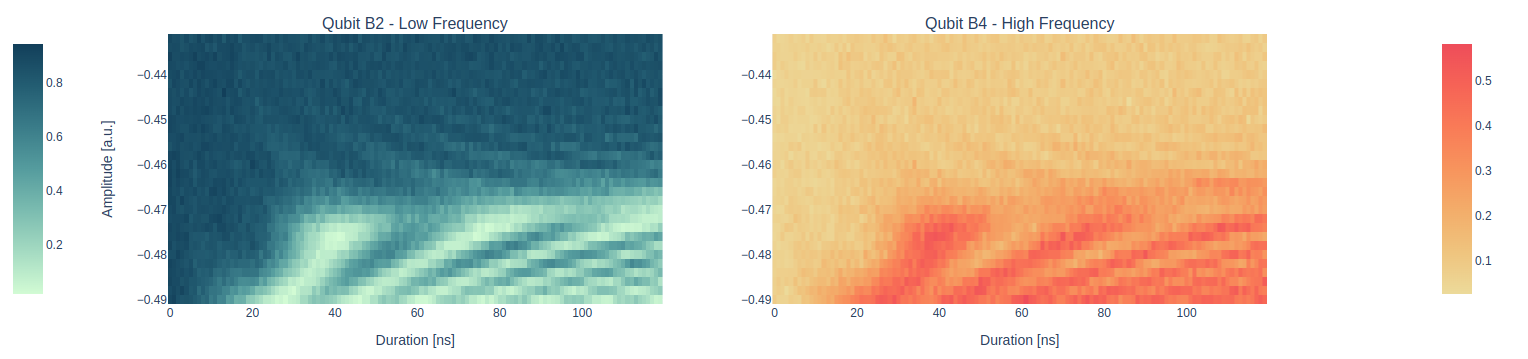
\includegraphics[width=\textwidth]{figures/B2B4_nofilter.png}
    \vfill
    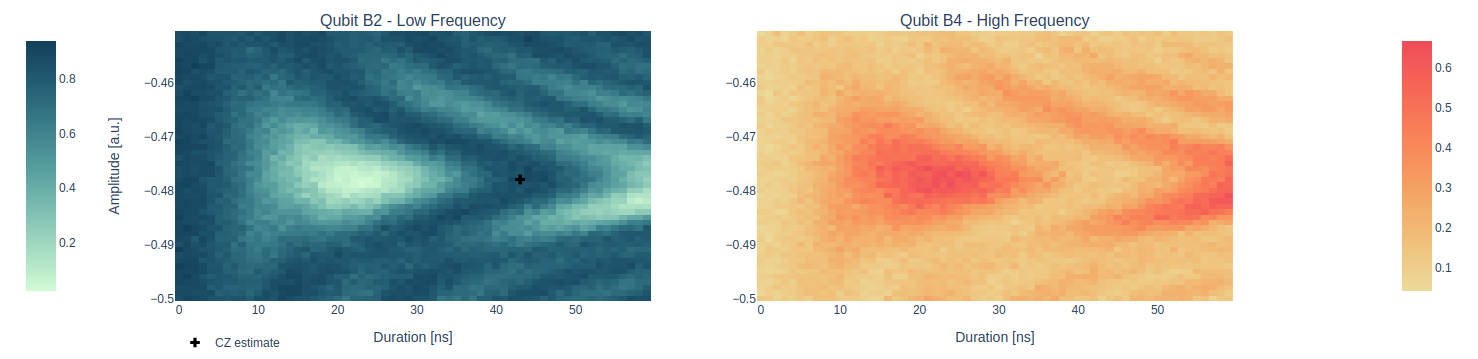
\includegraphics[width=\textwidth]{figures/B2B4.png}
  \end{figure}
\end{frame}

\begin{frame}{Cryoscope routine}
  \centering
  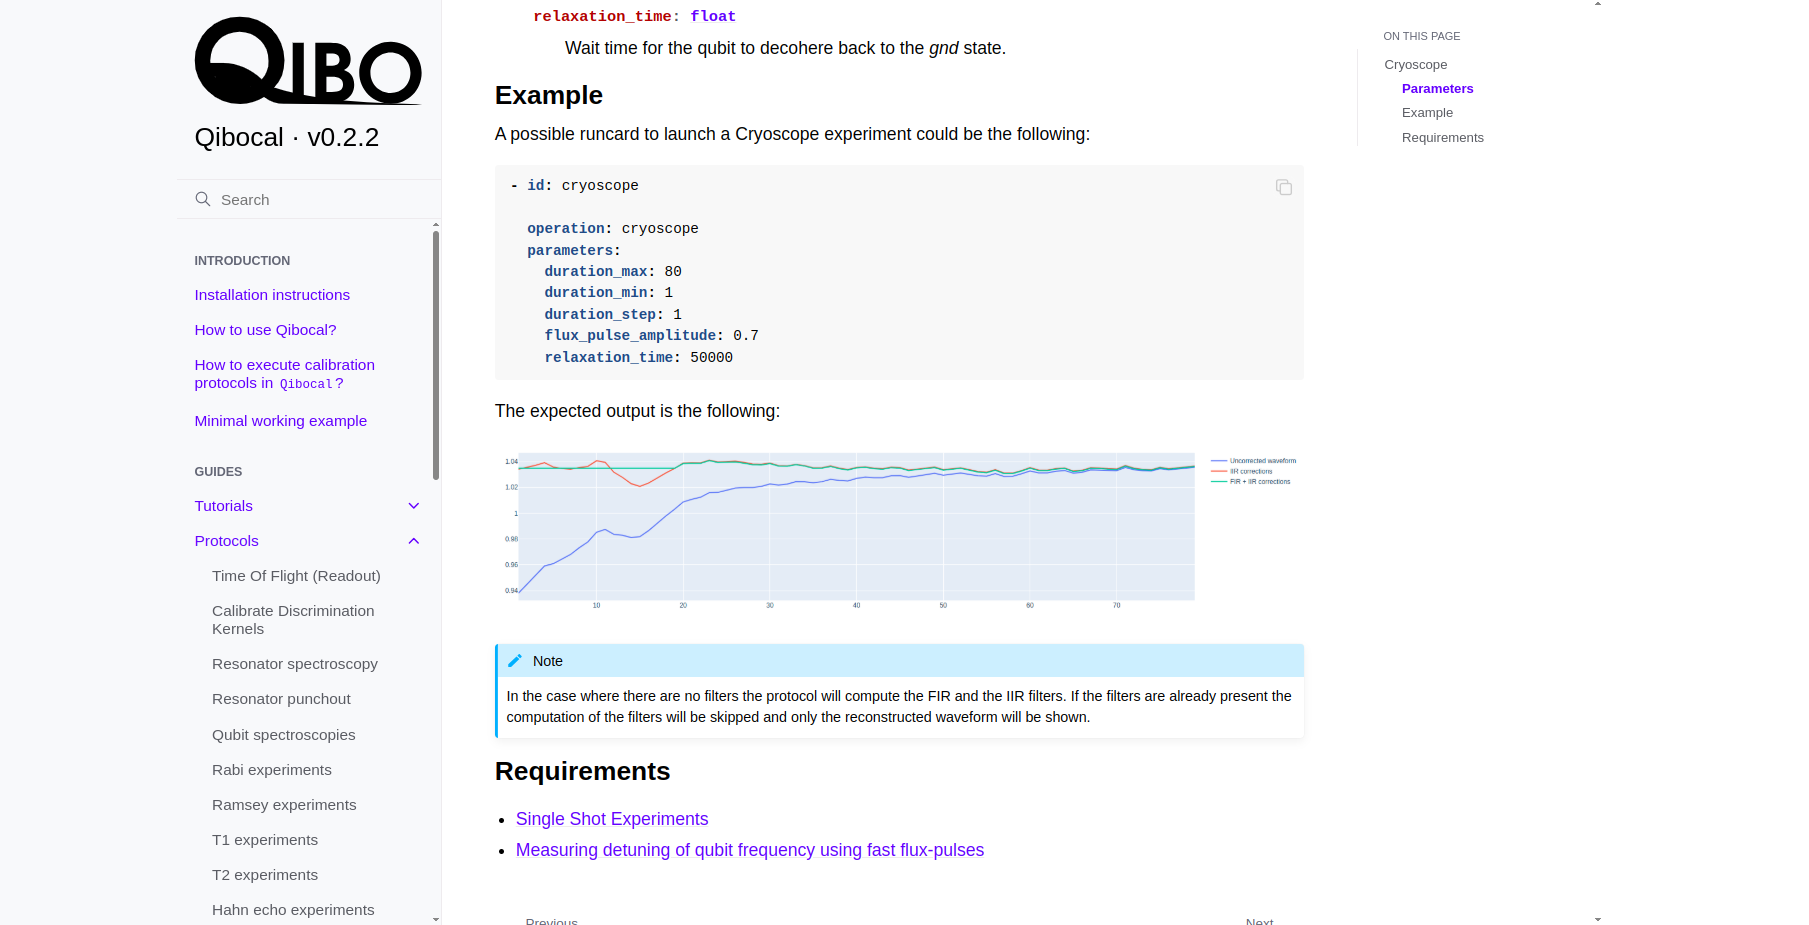
\includegraphics[height=\textheight]{figures/cryoscope_routine.png}
\end{frame}


\section{Conclusions \& Outlooks}

\begin{frame}{Conclusions \& Outlooks}
  \begin{itemize}[label={\raisebox{0.2ex}{\tiny$\bullet$}}]
    \item Tested automated optimization routines to enhance single-qubit Clifford gates fidelities and highlighted main limitations for systematic application
    \item Possible future work related to parameters optimization of the RB protocol itself for this purpose
    \item Extended Qibolab and Qibocal to support native $R_X(\pi/2)$ gates with dedicated calibration routines
    \item Implemented and added the Cryoscope calibration experiment to Qibocal library 
    \item Other possible experiments that can be added to Qibocal library include readout optimization, active qubit reset schemes, and leakage mitigation techniques 
  \end{itemize}
\end{frame}

\begin{frame}[t,standout]
\Large
Thank you
\end{frame}


\begin{frame}{References}
    \printbibliography
\end{frame}


\section*{Backup slides}

\begin{frame}{What is for?}
  \begin{columns}
    \begin{column}{0.5\textwidth}
      \begin{itemize}[label=\textbullet]
        \item \textbf{Simulation of quantum system:} "Nature isn't classical, dammit, and if you want to make a simulation of nature, you'd better make it quantum mechanical, and by golly it's a wonderful problem, because it doesn't look so easy"
                 %\href{https://link.springer.com/article/10.1007/BF02650179}{\faBook\,\, Richard Feynman, 1982, Simulating Physics with Computers}
        \item Optimization and modeling (chemistry, finance, traffic, weather...), eg. VQE, QAOA
        \item Quantum Algorithms 
        \item Quantum Machine Learning
      \end{itemize}
      \end{column}
      \begin{column}{0.5\textwidth}
        \begin{center}
            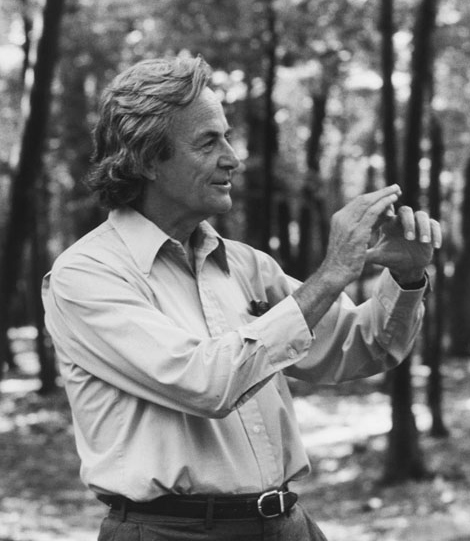
\includegraphics[width=0.8\textwidth]{figures/feynmann.jpg}
        \end{center}
      \end{column}
  \end{columns}
\end{frame}

\begin{frame}{Qubit platforms}
  \begin{center}
      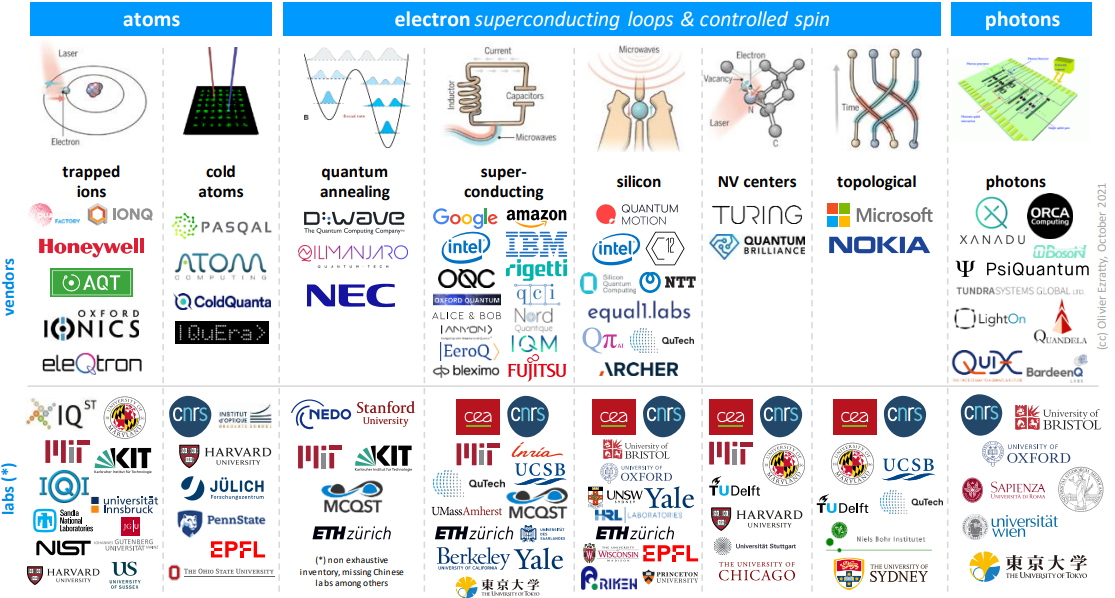
\includegraphics[height=0.82\textheight]{figures/platforms.png}
  \end{center}
\end{frame}

\begin{frame}[fragile]{Standard Randomized Benchmarking protocol}
    \begin{columns}
      \begin{column}{0.5\textwidth}
        RB protocol
      {\setbeamertemplate{enumerate items}[default]
       \begin{enumerate}[leftmargin=*, label=\arabic*.]
         \item Initialize the system in the ground state
         \item For each sequence length $m$ draw a sequence of Clifford group elements
         \item Calculate the inverse gate 
         \item Measure sequence and inverse gate
         \item Repeat the process for multiple sequences of the same length while varying the length
       \end{enumerate}}
      \end{column}
      \begin{column}{0.5\textwidth}
        RB features
        \begin{itemize}
          \item robust to SPAM errors
          \hspace{10mm}
          \item faster than state tomography
          \hspace{10mm}
          \item hardware-agnostic 
        \end{itemize}
      \end{column}
    \end{columns}
\end{frame}

\begin{frame}{Clifford gates}
  \begin{columns}
    \begin{column}{0.4\textwidth}
      \begin{itemize}[label=\textbullet]
        \item Special subset of quantum gates that map Pauli operators to Pauli operators under conjugation
        \hspace{10mm}
        \item Clifford gates group is generated by $H$, $S$, ($CNOT$) gates
        \hspace{10mm}
        \item Quantum circuits that consist of only Clifford gates can be efficiently simulated with a classical computer (Gottesman–Knill theorem)
      \end{itemize}
    \end{column}
    \begin{column}{0.6\textwidth}
      \begin{figure}
        \centering
        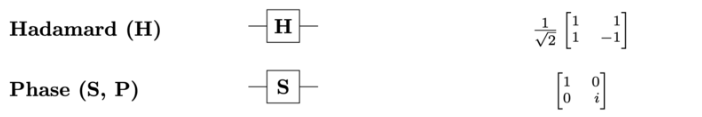
\includegraphics[width=\textwidth]{figures/HS.png}
        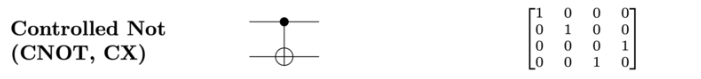
\includegraphics[width=\textwidth]{figures/CNOT.png}
        \vfill
      \end{figure}
    \end{column}
  \end{columns}
\end{frame}


\end{document}
